
As seen before in sec \ref{sec:tau_lepton}, when a $\tau$ is produced in a collision, it can decay into several different final states.
Hadronic final states, denoted \tauh, represent about 65\% of tau decays.
These hadronic final states are characterized by one or three charged hadrons with or without \pizero . But similar particles can be reconstructed from other processes and decays, such as events involving QCD jets.
Since these QCD jets greatly outnumber \tauh in the final states of proton-proton collisions at the LHC, \tauh identification algorithms have been designed in CMS to reject QCD jets as much as possible while keeping a \tauh identification efficiency somewhere between 35\% and 70\%, depending on the purity needed by the analyses. Identification algorithms classify all reconstructed jets as either background which means QCD jets, or signal which means \tauh decay products.
The standard \tauh identification algorithm used in CMS, which will be detailed in section \ref{sec:std_tau_id}, have reached excellent performance thanks to the use of particle-flow reconstruction but do not use its full potential. 

Deep learning algorithms have shown an ability to use available information as efficiently as possible for the task they are trained for. In the field of particle physics, for example, their use in heavy flavour jet-tagging \cite{btagging_NN} has shown significant improvements over previously used techniques. These networks show best results when their design, or architecture, simplifies the task at hand. New architectures specifically intended for high energy proton-proton collisions have shown promising results. One such architecture is the Recursive Neural Network (RecNN) \cite{Louppe:2017ipp} used to identify boosted jets originating from hadronically decaying W bosons. Deep learning techniques will be introduced by level of complexity leading to the RecNN in section \ref{sec:NN}. This architecture has been adapted to \tauh identification, as it is a similar task. The adaptations of this architecture as well as some improvements that have been implemented will be presented in section \ref{sec:RecNN}, along with the reached performance.

\section{The standard CMS hadronic $\tau$ decays identification}
\label{sec:std_tau_id}
\subsection{Decay mode finding}

First, the particles of the reconstructed jet are fed as input to the hadrons-plus-strip (HPS) algorithm \cite{tauh_reconstruction} to reconstruct and identify \tauh candidates. A first selection is the requirement that reconstructed jets have $\pt > 14\,\mathrm{GeV}$ and $|\eta| < 2.5$.
The constituent particles are combined into \tauh candidates compatible with one of the main $\tau$ decay modes, $\tau^- \rightarrow h^- \nu_\tau$, $\tau^- \rightarrow h^- \pizero \nu_\tau$, $\tau^- \rightarrow h^- \pizero \pizero \nu_\tau$, $\tau^- \rightarrow h^- h^+ h^- \nu_\tau$, and charge conjugates. The decay mode $\tau^- \rightarrow h^- h^+ h^- \pizero \nu_\tau$ is not considered owing to its relatively small branching fraction and high contamination from quark and gluon jets.

The \pizero produced in some decay modes have a mean life of about $9 \times 10^{-17}\,\mathrm{s}$ and about $99\%$ of their decays lead to two photons. Because of the large amount of material in the tracker, illustrated in Figure \ref{fig:tracker_material}, photons often convert before reaching the ECAL. The resulting electrons and positrons can be identified as such by the PF algorithm or, in the case their track is not reconstructed, as photons displaced along the $\phi$ direction because their trajectory is bent by the magnetic field.
These neutral pions are therefore obtained by adding iteratively reconstructed photons and electrons located in a strip of size $0.05 \times 0.20$ in the ($\eta$,$\phi$) plane:
\begin{itemize}
    \item Every reconstructed electrons and photons of $\pt > 0.5\,\mathrm{GeV}$ in the strip are added iteratively from highest to lowest \pt.
    \item At every step, the position of the center of the strip is re-computed as a \pt-weighted average of the position of all constituents.
    \item Any electron or photon not included in an existing strip is used as seed to another new strip.
\end{itemize}

\tauh candidates are then formed by creating all combinations of either one or three charged-particle and up to two strips in the jet.
Each \tauh candidate is then required to have a mass compatible with its decay mode and to have unit charge.
Collimation of the products are ensured by requiring all charged hadrons and neutral pions to be within a circle of radius $\Delta R = (2.8\,\mathrm{GeV})/\pt$ in the ($\eta$,$\phi$), which is called the signal cone.
The size of the signal cone is, however, not allowed to increase above 0.1 at low \pt, nor to decrease below 0.05 at high \pt. It decreases with \pt to account for the boost of the $\tau$ decay products. Finally, the highest \pt selected \tauh candidate in a given jet is retained. The four-momentum of the \tauh candidate is determined by summing the four-momenta of its constituent particles.

\subsection{Isolation}


\tauh candidates reconstructed from QCD jets are likely to be surrounded by other particles coming from the jet.
Isolation is therefore a powerful way to reject background QCD jets.

Two approaches are available : cut-based and multi-variate.

\paragraph{Cut-based} Isolation is computed from the \pt sum of charged particles and photons with $\pt > 0.5$ GeV within an isolation cone of $dR=0.5$ centered around the \tauh direction, excluding particles used to form the \tauh candidate. In order to mitigate pileup contribution, tracks associated to the considered charged particles are required to be compatible with the \tauh production vertex within a distance $\Delta z < 0.2\,\mathrm{cm}$ and $\Delta r < 0.03\,\mathrm{cm}$. The contribution from pileup is estimated as $\Delta \beta$ calculated from the contribution of charged displaced particles and removed as
\begin{equation}
    I_{\tau} = \sum_{charged, \Delta z<0.2 cm} \pt + max \Big\{ 0, \sum_{\gamma} \pt - \Delta\beta \Big\} \msep
    \label{eq:isolation}
\end{equation}
\begin{equation}
    \Delta \beta = 0.46 \sum_{charged,\Delta z>0.2 cm} \pt \mend
\end{equation}
Working points are defined by the thresholds on the value taken by the isolation defined in equation \ref{eq:isolation}. Usual working points such as loose, medium, tight are thresholds are 2.0, 1.0 and $0.8\,\mathrm{GeV}$ respectively.

\paragraph{Multi-variate} This method is based on decision trees. These are machine learning techniques that rely on finding the best successive cuts on the available variables to separate signal and background in a training set. Boosting is a method of combining many weakly classifying trees into a strong classifier. A BDT is trained on an appropriate choice of isolation variables to give best separation between QCD jets and \tauh : 
    \begin{itemize}
        \item charged- and neutral-particle isolation sums defined as in eq \ref{eq:isolation}.
        \item The reconstructed decay mode.
        \item the transverse impact parameter $d_0$ of the leading tack of the \tauh candidate and its significance $d_0 / \sigma_{d_0}$
        \item the distance between the $\tau$ production and decay vertices, $|\Vec{r}_{SV} - \Vec{r}_{PV}|$, and its significance $|\Vec{r}_{SV} - \Vec{r}_{PV}|/\sigma_{|\Vec{r}_{SV} - \Vec{r}_{PV}|}$, along with a flag indicating whether a decay vertex has successfully been reconstructed for a given \tauh candidate. The positions of the vertices, $\Vec{r}_{SV}$ and $\Vec{r}_{PV}$, are reconstructed using the adaptive vertex-fitter algorithm \cite{Waltenberger_2007}.
        \item More details on the variables can be found in \cite{tauh_reconstruction}.
    \end{itemize}

\subsection{Anti-leptons discriminants}

Electrons and muons can easily be misidentified as \tauh, particularly in the $h^{\pm}$ decay mode. Electrons radiating a bremsstrahlung photon that subsequently converts may also get reconstructed in the $h^{\pm}\pizero$ decay mode. Therefore, discriminants have been developed to separate such leptons decays from real \tauh decay products.

Electrons are rejected by a BDT using observables that quantify the distribution in energy depositions in the ECAL and HCAL, in combination with observables sensitive to the amount of bremsstrahlung emitted along the leading track. The BDT also uses observables sensitive to the overall particle multiplicity, to distinguish electromagnetic from hadronic showers.
All these variables are listed in \cite{tauh_reconstruction}.
    
Muons are rejected by requiring that no track segments are found in at least two muon stations within a cone of size $\Delta R = 0.3$ around the \tauh direction. \tauh candidates are also rejected when the sum of the energies in the ECAL and HCAL corresponds to less than 20\% of the momentum of their leading track.

\subsection{Simulation of QCD jets and hadronic $\tau$ decays}
\label{sec:NN_datasets}

In order to compare the both classification methods, their performance is expressed in terms of signal efficiency and background rejection. To quantify these, and to provide a training set for our deep learning algorithm, datasets of QCD jets and hadronic tau decays have been selected from the simulated CMS datasets that were introduced in \ref{sec:cms_physics_event_generation}. Instead of simulating isolated QCD jets and \tauh separately, entire collision events are used as they provide a realistic environment similar to the one in which the classifier will be used.

Selected processes leading to \tauh and QCD jets in the final state are detailed in table \ref{tab:NN_b_s_diff}. QCD jets are obtained from QCD multijet events in which true \tauh are extremely rare, while \tauh are taken from events with true taus in the final state (MSSM $H\rightarrow \tau\tau$, DY $Z\rightarrow \tau\tau$).


The proton-proton collision events are generated with PYTHIA 8 \cite{SJOSTRAND2008852}, and are then processed by the CMS GEANT4 simulation, as detailed in section \ref{sec:cms_physics_event_generation}. The generation-level information is kept and will be referred to as gen level. All the information coming out of the detector simulation is fed to the CMS reconstruction algorithms, where the particle flow algorithm provides the list of reconstructed stable particles. Higher-level objects such as jets, are reconstructed by combining these particles using the clustering algorithms introduced in \ref{sec:jet_clustering}.

As stated before, the identification of \tauh and QCD jets is performed jet by jet. A reconstructed jet is defined as signal if it is selected from the genuine tau samples, and as background if selected from the QCD multijet samples. To ensure purity, some extra cuts are applied, these cuts can be found in table \ref{tab:NN_b_s_diff}.

The matching between reconstructed jets and gen level \tauh is done by ensuring their respective directions are aligned. This is done by requiring the distance separating their orientation in the ($\eta ,\phi$) plane to be $\Delta R < 0.1$.


\begin{table}[ht]
    \caption{Provenance and cuts applied to reconstructed jets defining signal and background.}
    \centering
    \begin{adjustbox}{max width=\textwidth}
    \begin{tabular}{c||c|c}
        & \tauh (signal) & QCD jets (background) \\
        \hline \hline
        \multirow{3}{*}{Hard processes} & SUSY ggH $\rightarrow\tau\tau$ & \multirow{3}{*}{\begin{minipage}{0.4\textwidth}QCD multijets samples ordered by \pt : 15-30, 30-50, 50-80, 80-120, 120-170, 170-300 \end{minipage}} \\
        \cline{2-2}
         & SUSY bbH to $\rightarrow\tau\tau$ & \\
        \cline{2-2}
         & DY to tautau & \\
        \hline
        phase-space cuts & \multicolumn{2}{c}{$20<\pt<100 \text{ and } |\eta|<0.8$}\\
        \hline
        specific extra cuts & matched with gen-level \tauh & any \\
        \hline
    \end{tabular}
    \end{adjustbox}
    \label{tab:NN_b_s_diff}
\end{table}

Parts of these sets are also going to be used in the training of the deep learning algorithm. But biases coming from the difference between signal and background distribution can cause mistraining. For example, if both background and signal samples had different \pt distribution, the network could wrongly assume that the \pt of a reconstructed jet is correlated to its nature as a \tauh or a QCD jet, which should be avoided. To prevent this bias, the signal and background jets are split by \pt bins, and the selection signal and background jets is done in each \pt bin.

\subsection{Performance}


\begin{figure}
    \centering
    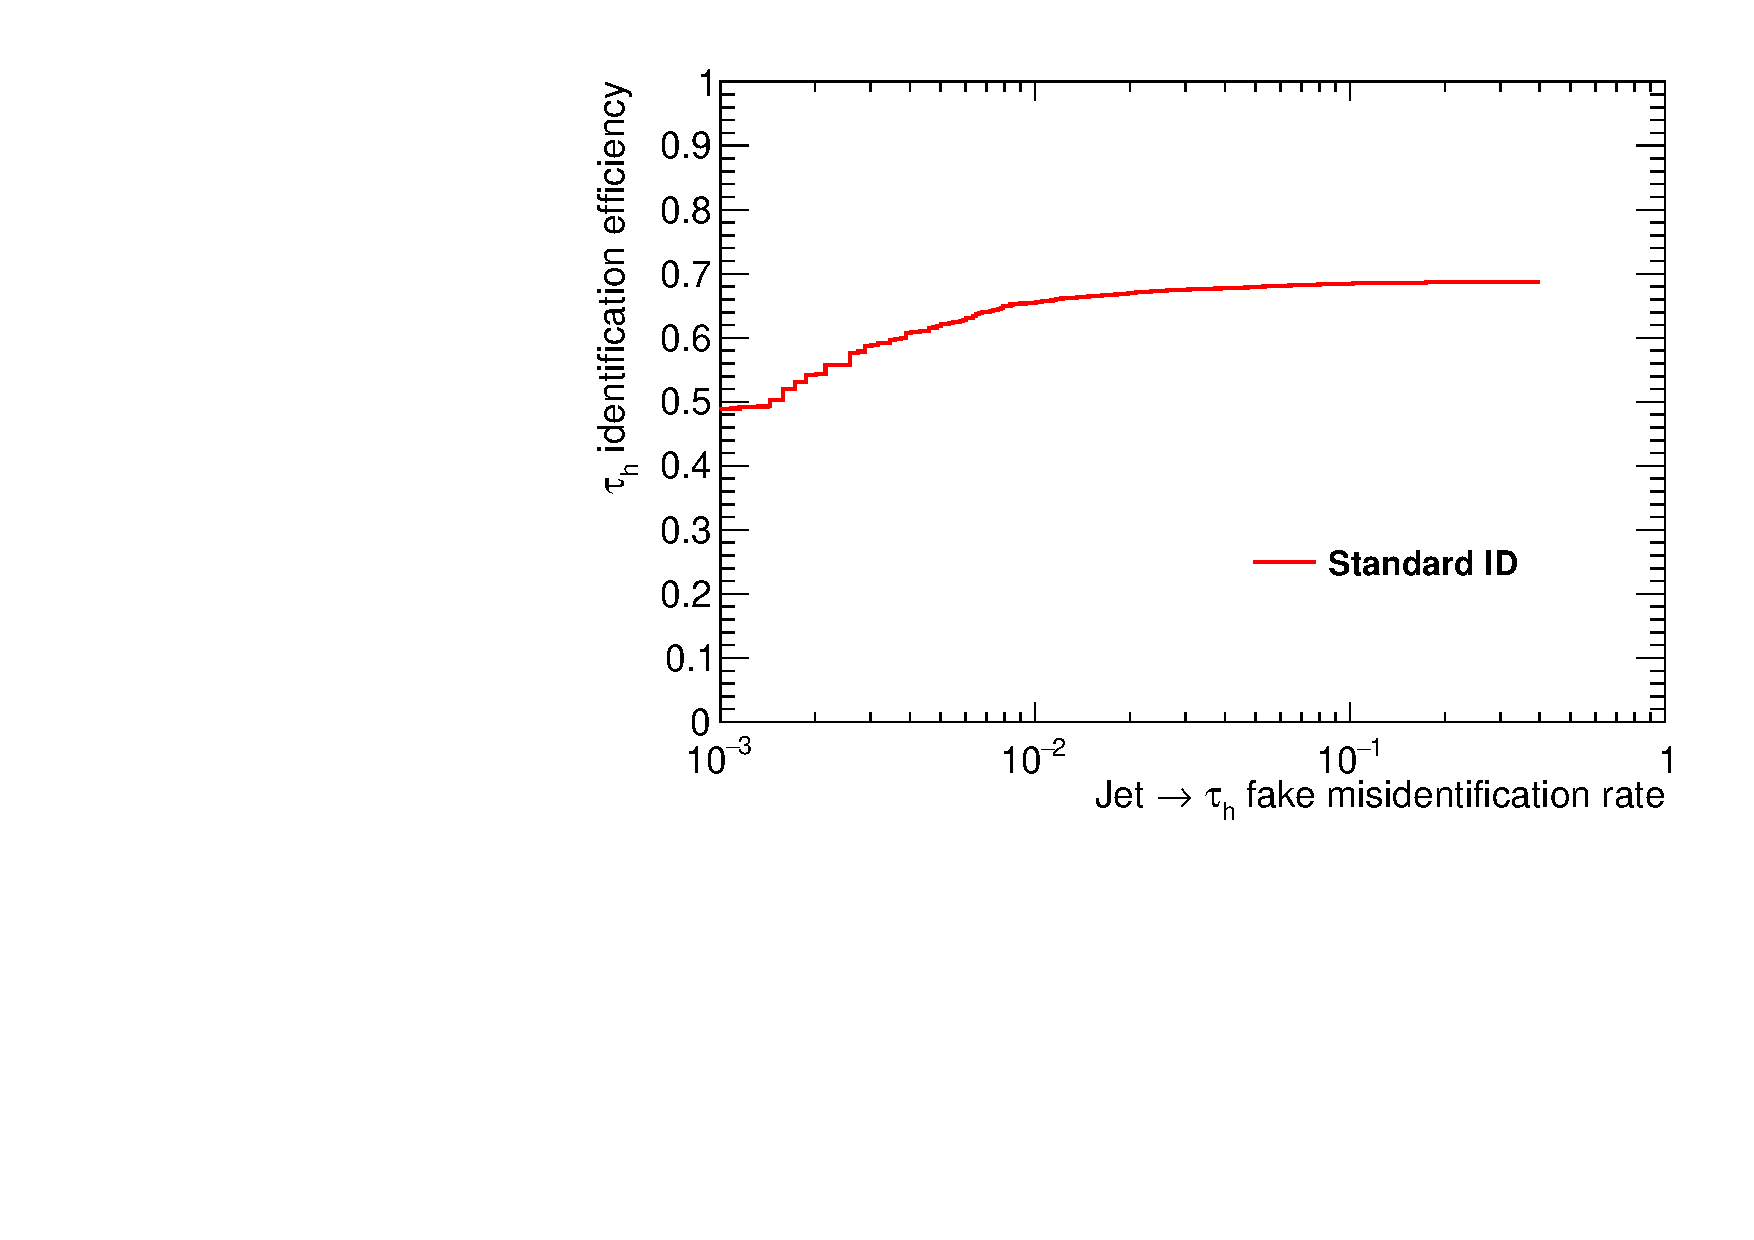
\includegraphics[width=\textwidth]{Images/ROC_comp_std.pdf}
    \caption{\tauh identification ROC curve for the standard method. The x axis is set to a logarithmic scale.}
    \label{fig:std_ROC}
\end{figure}

Performance is evaluated in terms of signal efficiency and background rejection. The signal efficiency is defined as the ratio of the number of well-tagged \tauh over the total number of \tauh in the selected population. The background rejection is similarly defined as the ratio of the number of well-tagged QCD jets over the total number of QCD jets in the population.

While the goal of a classifier is to tag objects as signal or background, most will instead provide with a score between 0 and 1. A score close to 0 is to be interpreted as very likely to be background, and a score close to 1 as very likely to be signal. This continuous score can then be translated into a discrete tag by the choice of a working point (WP) value. For a given WP, every reconstructed jet that scores below the WP value is then tagged as QCD jet, and every reconstructed jet that scores higher is tagged as \tauh. The values of the signal efficiency and background rejection can be measured for a continuous scan of WP values. The created curve in the signal efficiency vs background rejection space is called a Receiver Operating Characteristic (ROC) curve. The standard identification ROC curve is shown in Figure \ref{fig:std_ROC}
A numerical figure of merit often used to quantify the overall performance of a classifier is the area under the ROC curve, called ROC AUC, as it is maximum when signal efficiency and background rejection is perfect.
In our case, ROC AUC might not be the best figure of merit, as it does not take into account which regions are best covered by the technique. Indeed, in our case the standard identification technique is based on applying hard cuts such as decay mode finding and anti-lepton discriminant before scanning the score of the isolation BDT. This is why the ROC of the standard technique reaches a plateau, as the plateau corresponds to maximum efficiency allowed by the previous cuts.

QCD jets are also overwhelmingly more present in collisions than \tauh, which means useful working points are in the region of high background rejection. 

\subsection{Intrinsic limitations}

The cut-based method relies on a single variable, namely isolation, to classify. The BDT-based method is an improvement on the cut-based method as it combines isolation with other variables susceptible to bring more information relevant to the classification process. But the BDT still takes a limited amount of information encoded into a strict number of variables. The construction of such variables do not take into account all the information gathered in the detection and reconstruction phases. A possible improvement should therefore be expected from using all the available information rather than a chosen subset. Deep learning techniques are conceptually adequate for such a task as they take all available information in and the process of such information is then completely derived from training.


\section{From a single neuron to recurrent networks}
\label{sec:NN}
Indeed, neural networks have revolutionized fields such as big data, image recognition, and even pseudo-data generation.
Neural networks are based on processing units called neurons. The combination of such neurons into networks allows a huge amount of information processing possibilities. Those neural networks are then trained to give the desired output by a trial and error process on a set of examples, called the training set. The possibilities gained by the complexity of a neural network comes with a need for a bigger training set, which can easily be obtained by simulation.

The organization of the neurons in the network is called architecture. Neural networks have shown their best achievements when their architecture are specifically designed for the task at hand.

\subsection{Basics : neurons, dense networks, deep learning}

\subsubsection{Neuron}

\begin{figure}
    \centering
    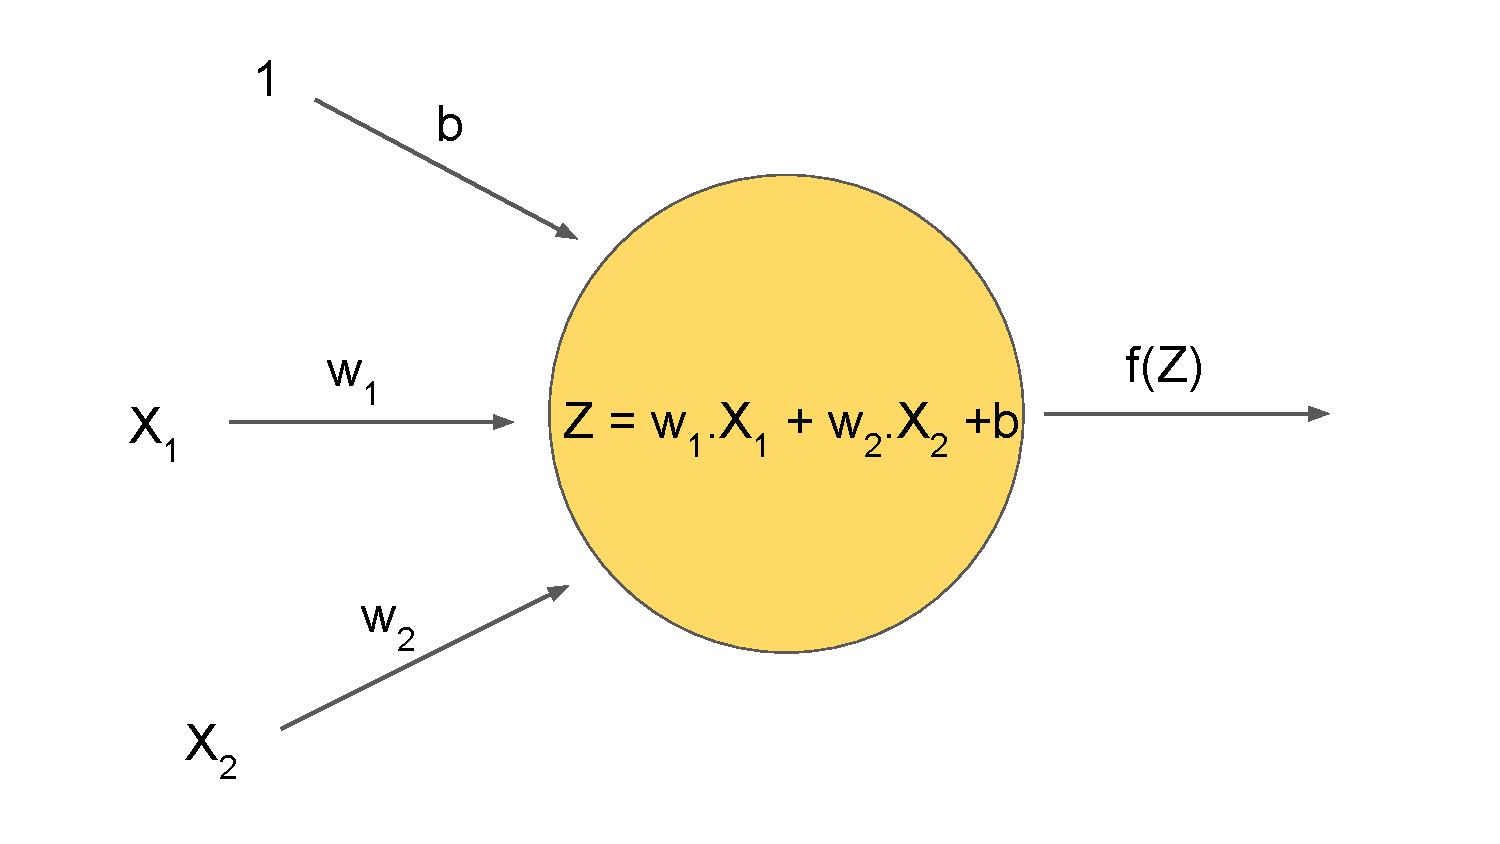
\includegraphics[width=0.8\textwidth]{Images/signle_neuron(1).pdf}
    \caption{Diagram of a single neuron, in the case of two input variables $X_1$ and $X_2$. The output of the neuron is $f$ is the activation function chosen for the neuron.}
    \label{fig:neuron_diagram}
\end{figure}


\begin{figure}
    \centering
    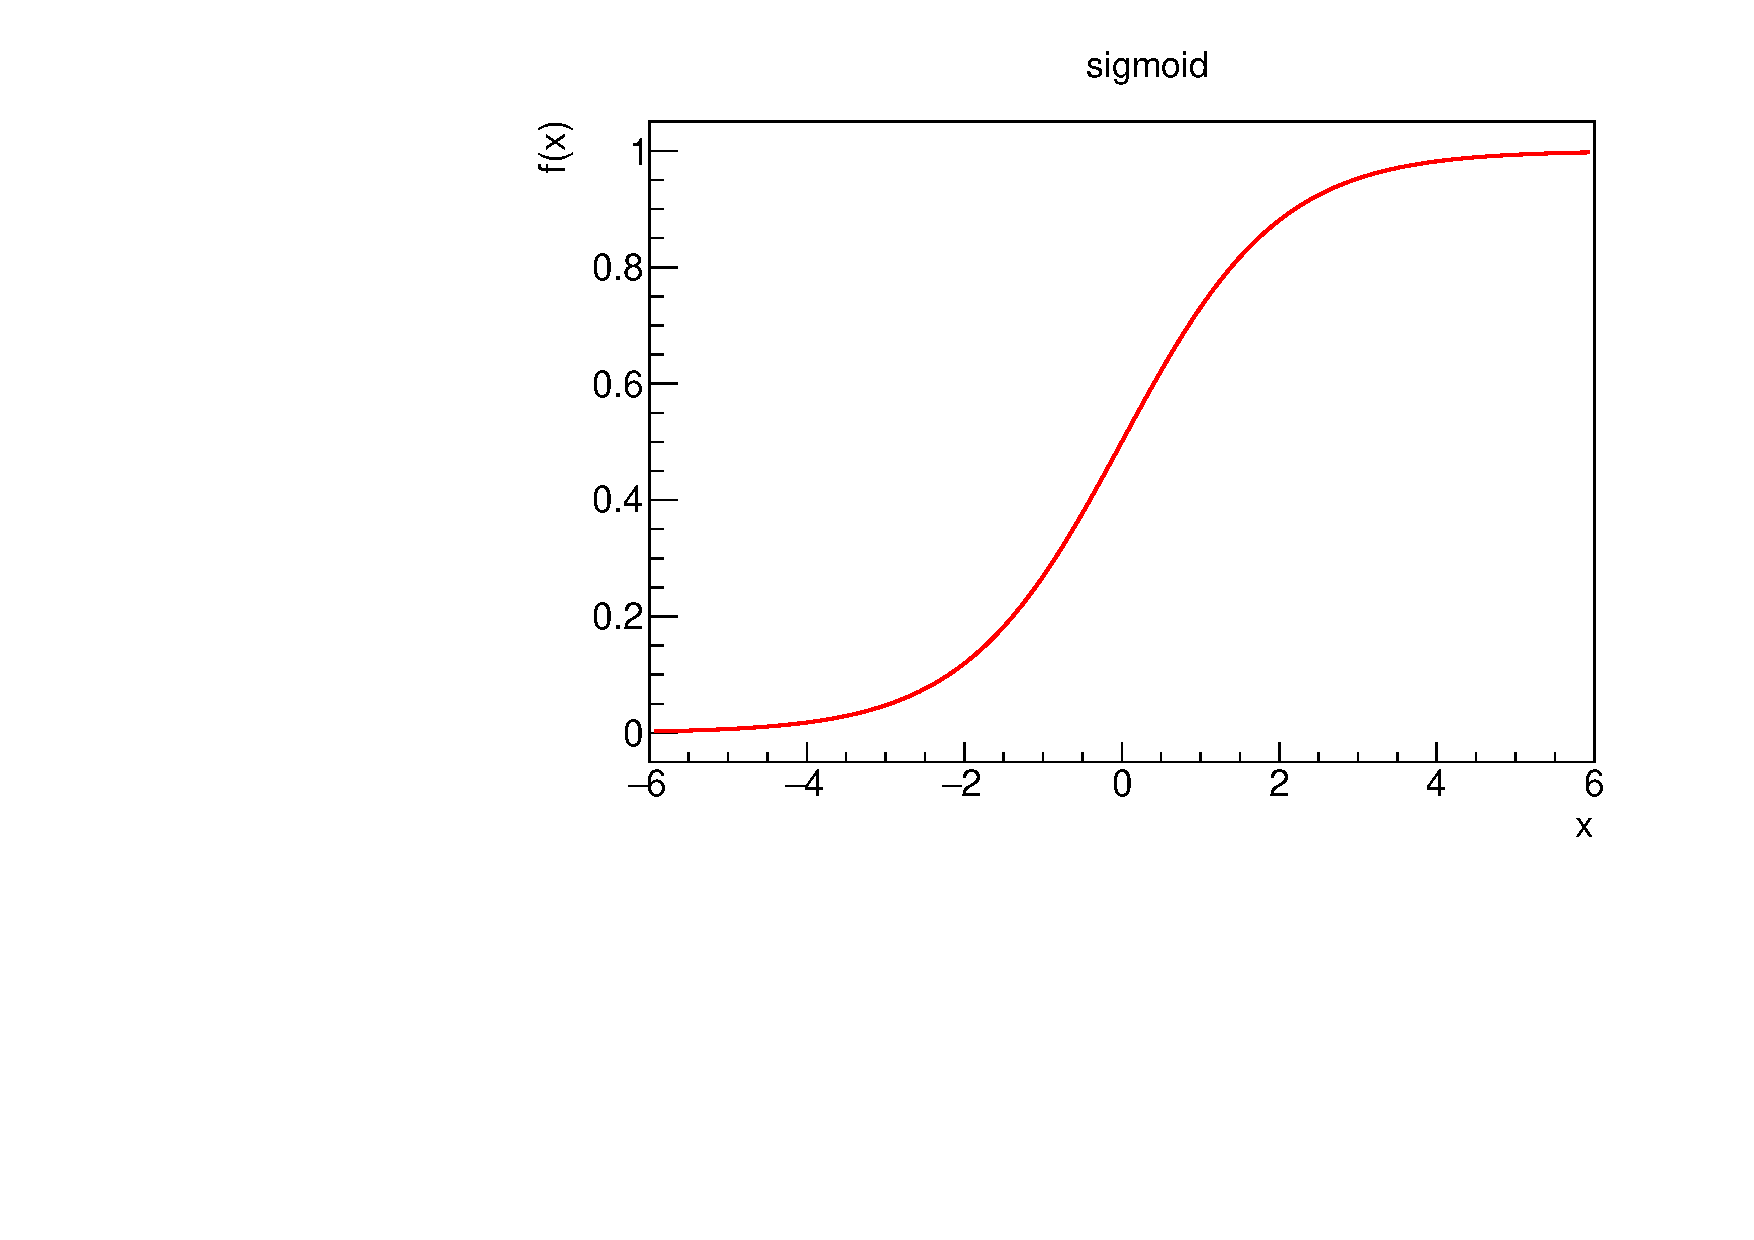
\includegraphics[width=0.45\textwidth]{Images/sigmoid.pdf}
    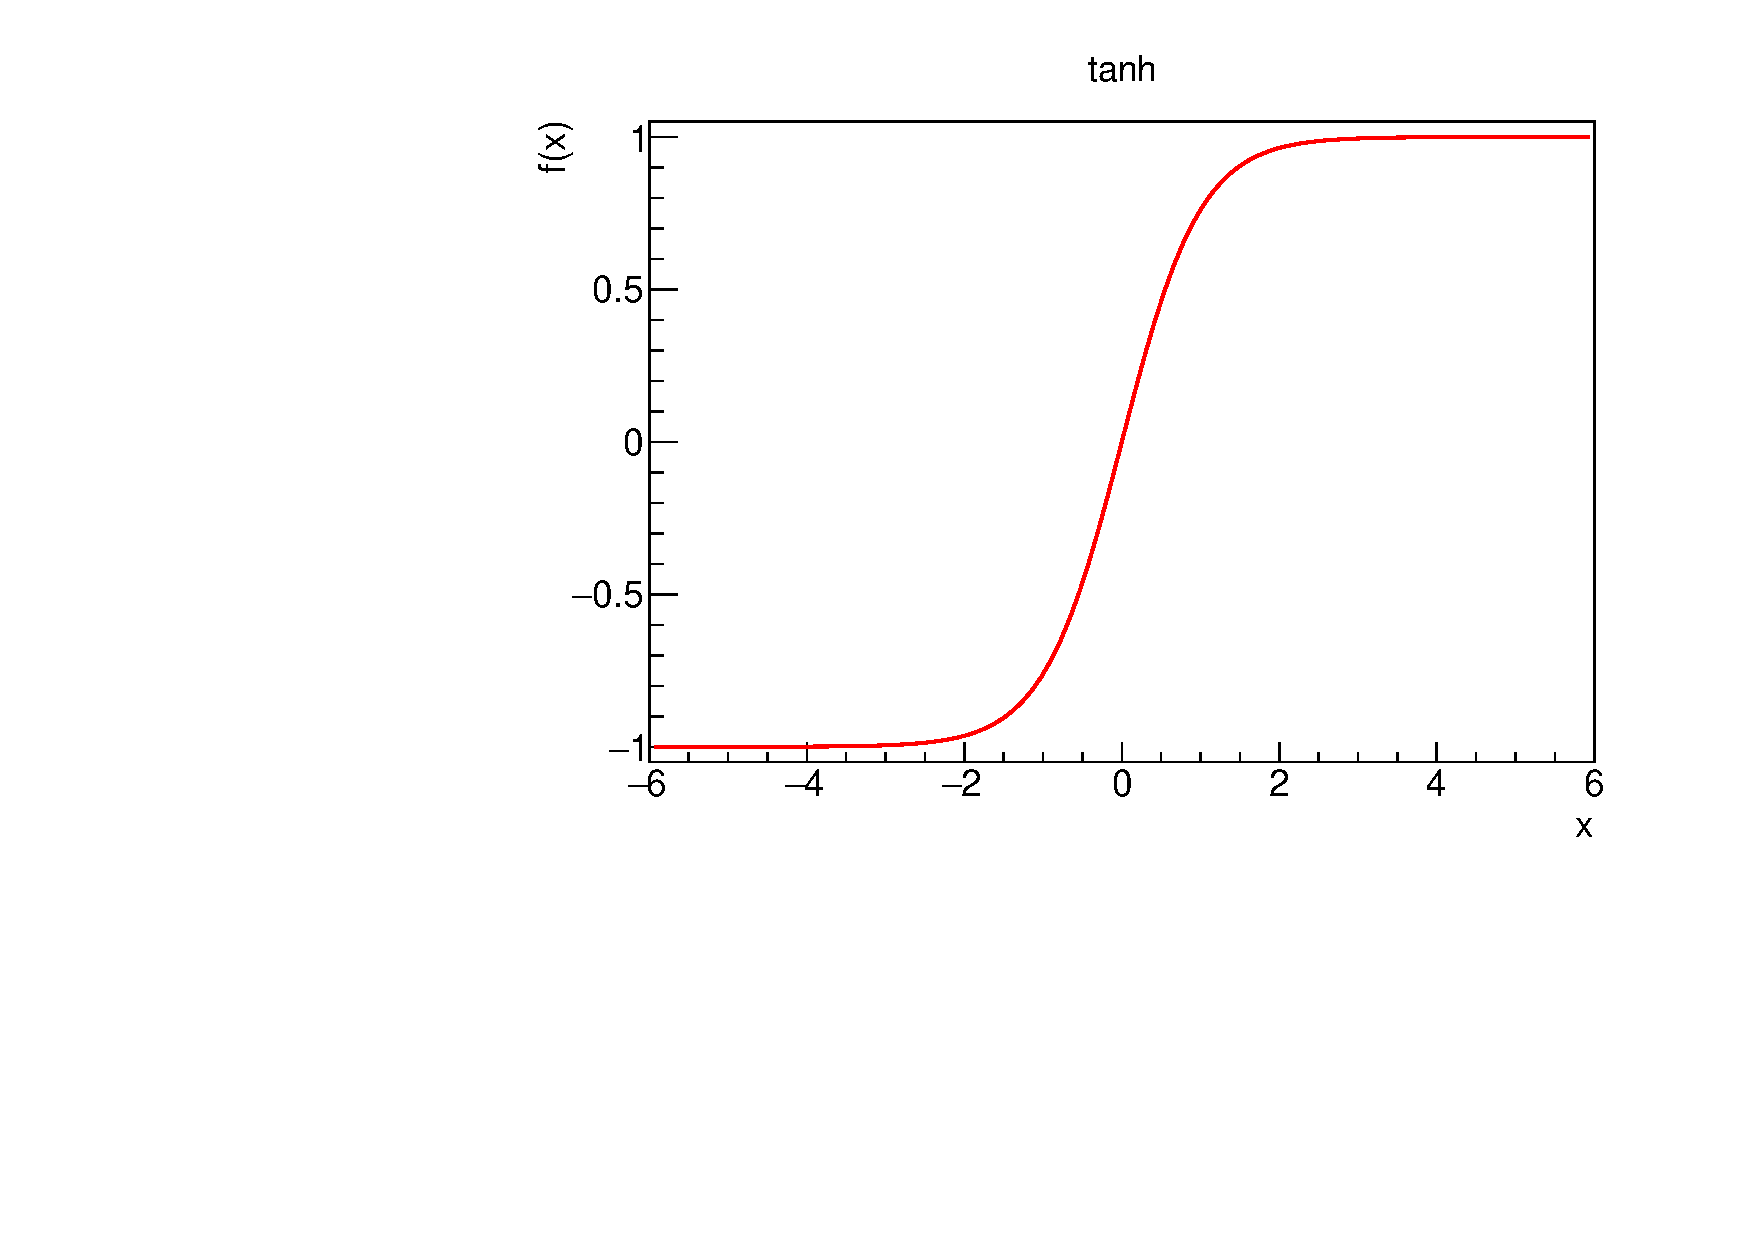
\includegraphics[width=0.45\textwidth]{Images/tanh.pdf}
    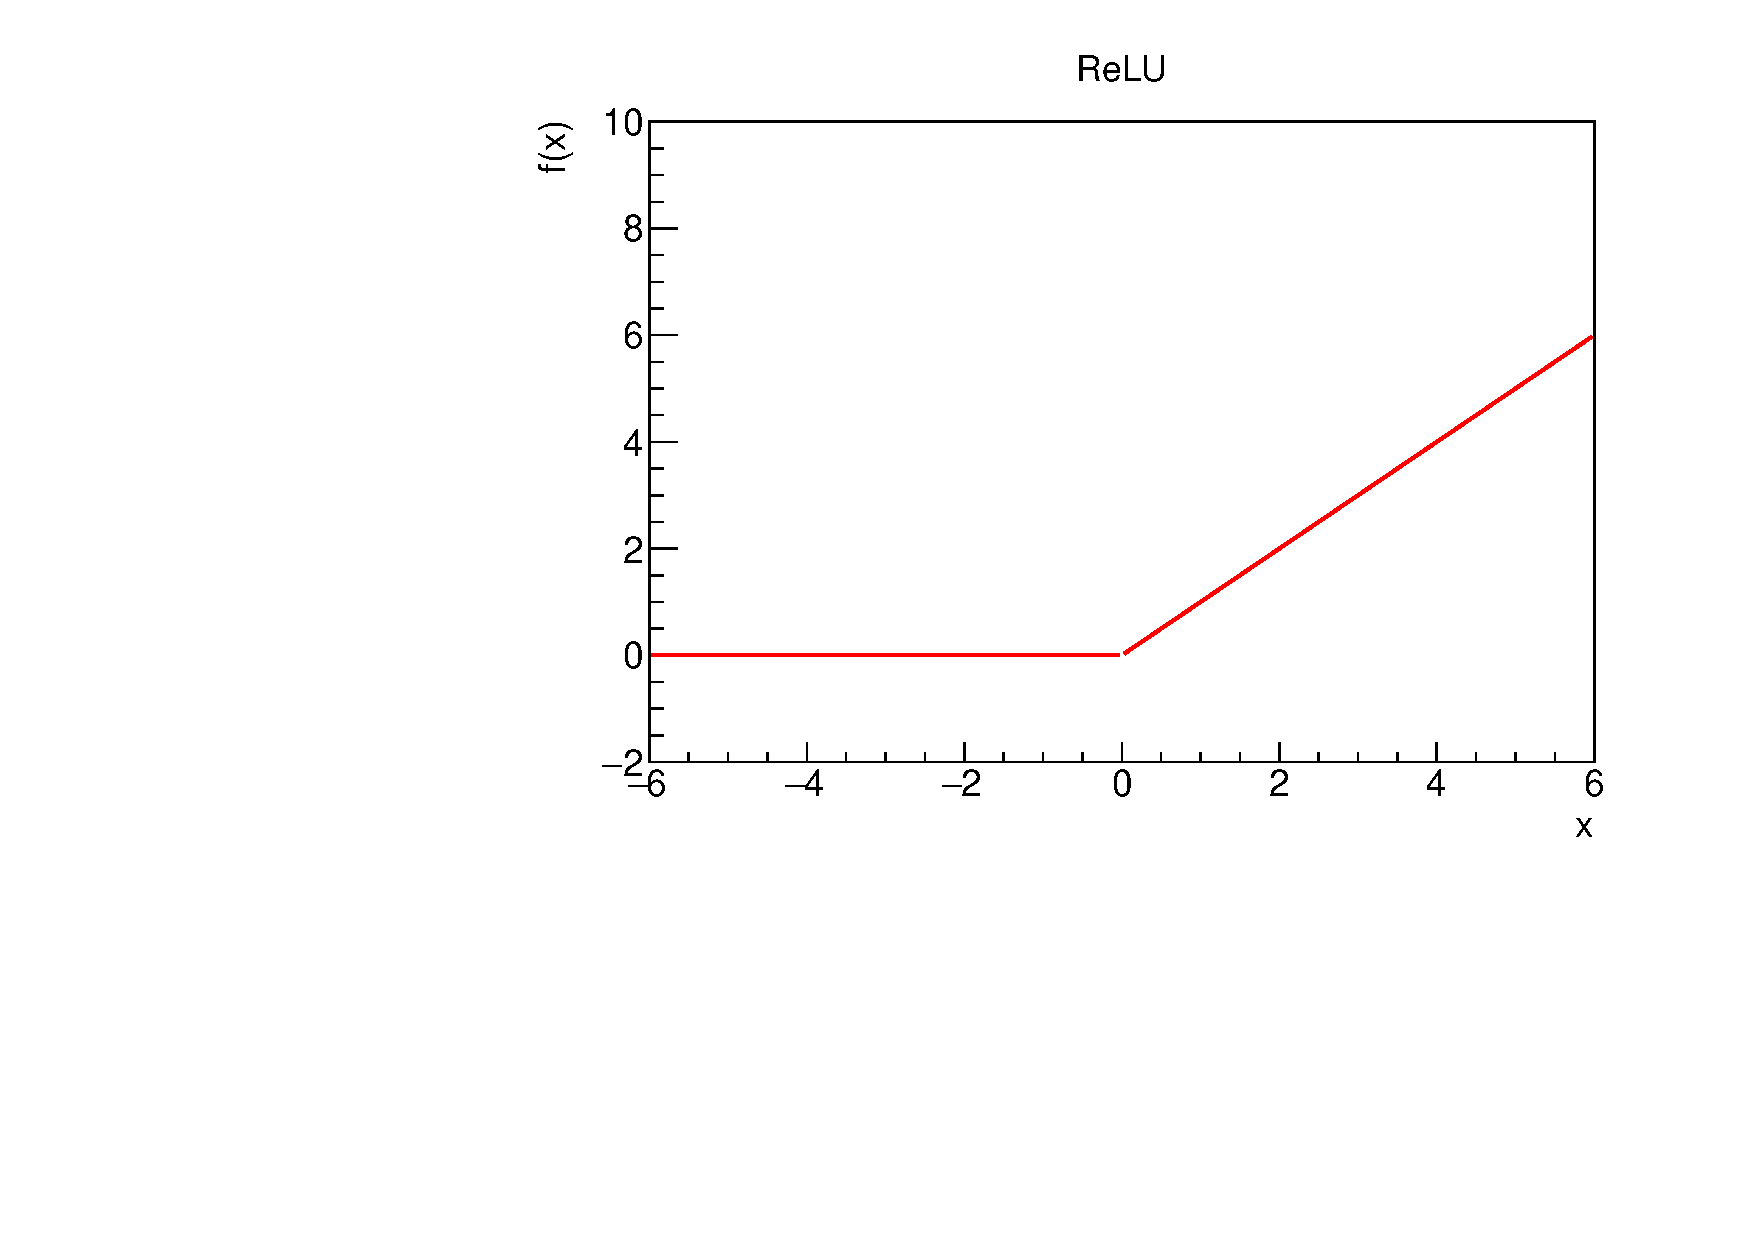
\includegraphics[width=0.45\textwidth]{Images/relu.pdf}
    \caption{Visualization of the used activation functions.}
    \label{fig:activation_functions}
\end{figure}

A neuron is defined by an activation function $f$, a set of scalar weights $w_i$, and a bias $b$. It takes a number of input variables denoted $X_i$. The layout of a neuron taking two inputs is illustrated in Figure \ref{fig:neuron_diagram}. First, the weighted output $z$ is defined as $z = \sum w_i\times X_i + b$. The output of the neuron is then $f(z)$. While the activation function can be any nonlinear function, the different activation functions used here are the sigmoid function
\begin{equation}
    f(x) = \frac{1}{1+e^{-x}} \msep
\end{equation}
the tanh function
\begin{equation}
    f(x) = \frac{2}{1 + e^{-2x}} -1 \msep
\end{equation}
and the ReLU function
\begin{equation}
    f(x) = \begin{cases} 0 &\text{for $x < 0$} \\ x &\text{for $x \geq 0$} \end{cases} \mend
\end{equation}
These functions are displayed in Figure \ref{fig:activation_functions}.

\subsubsection{Densely connected network}


\begin{figure}
    \centering
    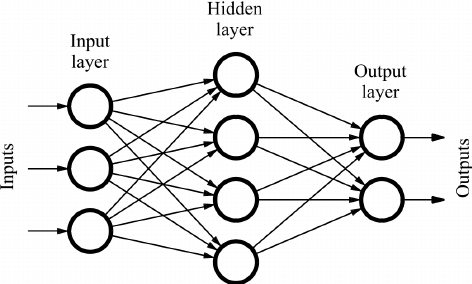
\includegraphics[width=0.5\textwidth]{Images/dense_network.png}
    \caption{Diagram of an example of a feed-forward densely connected network with 3 input variables, 4 neurons in the hidden layer and 2 output neurons.}
    \label{fig:dense_network}
\end{figure}

A network is created from neurons by connecting their inputs and outputs. A simple case is the feed-forward densely connected network, such as the one shown in Figure \ref{fig:dense_network}. In this architecture, neurons are organized by layers. The output of each neuron in a given layer is are sent to all neurons in the next layer. The inputs of the first layer are the input variables. The information then propagates through the evaluation of the neurons in each layer. The output of the last layer is then the output of the network for the given set of inputs, in other words the example data. An architecture is called feed forward when there is no cycle in the propagation of the evaluation from inputs to outputs. Such an architecture creates the possibility of approximating theoretically any function of the inputs, as stated by the universal approximation theorem \cite{Cybenko1989}, as long as the activation functions used in the neurons are nonlinear.

\subsubsection{Training: loss function and backpropagation}

In order to find the set of weights and biases that allows the network to perform the desired task, the network is trained.
As previously mentioned, the training phase relies on a set of examples of inputs associated with their target output value. The training is done iteratively. The first step is comparing the output of the network for a set of input variables to the desired target output. This comparison is quantified through the use of a metric called the loss function. The loss function is required to be a differentiable function and is designed to reach a minimum when the output is equal to the target value. Training the network to perform the task is therefore equivalent to finding the network parameters (weights and biases) that minimize the value of the loss function for the whole training set, provided the training set is a representative sample of the global population.

But the space of configurations for the weights and biases of the network has a huge dimensionality. The iterative process of training the network case by case can then lead to stagnation if examples are evaluated and parameters adapted for each example of the training set. To avoid this stagnation, the parameters are changed to minimize the average of the loss function over a number of examples, called a mini-batch. The number of examples in each mini-batch is referred to as the mini-batch size.

The way the parameters are changed to minimize the loss function depends on which optimizer algorithm is used. Most optimizers rely on backpropagation, which means the variation that should undergo a parameter is computed by propagating the change of the loss function backwards through all the layers of neurons between the output of the network and the considered neuron \cite{1986Natur.323..533R}.


A classical problem that can occur in the training of neural networks is the existence of local minima of the loss function. Indeed, local minima can lead to a sub-optimal training, as it prevents the network from reaching a potentially lower global minimum. To mitigate such effects, diminishing learning rates as well as momentum-based optimizers are used. The learning rate is a simple scalar that multiplies the changes in parameters for a given change in loss. By starting at a high value of this learning rate, it is possible to avoid local minima that are too small. After several iterations of training, this rate can be lowered to help reach the lowest point of the minimum. Momentum-based optimizers try to avoid minimums by multiplying the learning rate by a factor proportional to the gain of the last step. Indeed, the more a training step helped minimizing the loss function, the bigger the next step, avoiding local minima on the way to a global minimum.

Backpropagation comes with another important problem called vanishing gradients. This is due to the change of output of a neuron being relatively small compared to change of its input. Indeed, an activation function such as the sigmoid, illustrated in Figure \ref{fig:activation_functions}, can lead to states where the derivative is close to 0. But to compute the update to a given parameter for a given neuron, backpropagation uses the derivatives of the activation functions of the neurons in the layers between the neuron and the output as factors. Thus, the more layers are in between a neuron and the final layer, the more likely it is that its parameters will update based on a derivative that is close to 0. In other words, this means that a change in the parameters of a neuron in an early layer will have a relatively small effect on the loss compared to a similar change in the last layers. This leads to a slower training of the early layers compared to the training of the last layers. Therefore, a very deep network will explore the space of its parameters very slowly compared to a shallow network. This can even lead to a stagnation of the overall performance, which means the network does not gain anything from training. This is mitigated by the use of an activation function such as the ReLU. This activation function mitigates the small derivative issue by having a much larger domain where the derivative is not close to zero. The use of cross-entropy as a loss function also allows to mitigate the vanishing gradients problem. Cross-entropy is defined as 
\begin{equation}
    f(y,\hat{y}) = -(y\,\mathrm{log}(\hat{y}) + (1-y)\,\mathrm{log}(1-\hat{y})) \mend
\end{equation}
where $y$ is the target output and $\hat{y}$ the output of the network. Indeed, the derivative of sigmoid activation functions cancels out in the computation of the derivative of the cross-entropy function with respect to a parameter of the network \cite{NN_book}. One can also mitigate further this problem by designing an architectural workaround, avoiding deep network when possible, for example using recurrent neural networks, which are introduced in the following section.

\subsection{Recurrent neural networks}

\begin{figure}
    \centering
    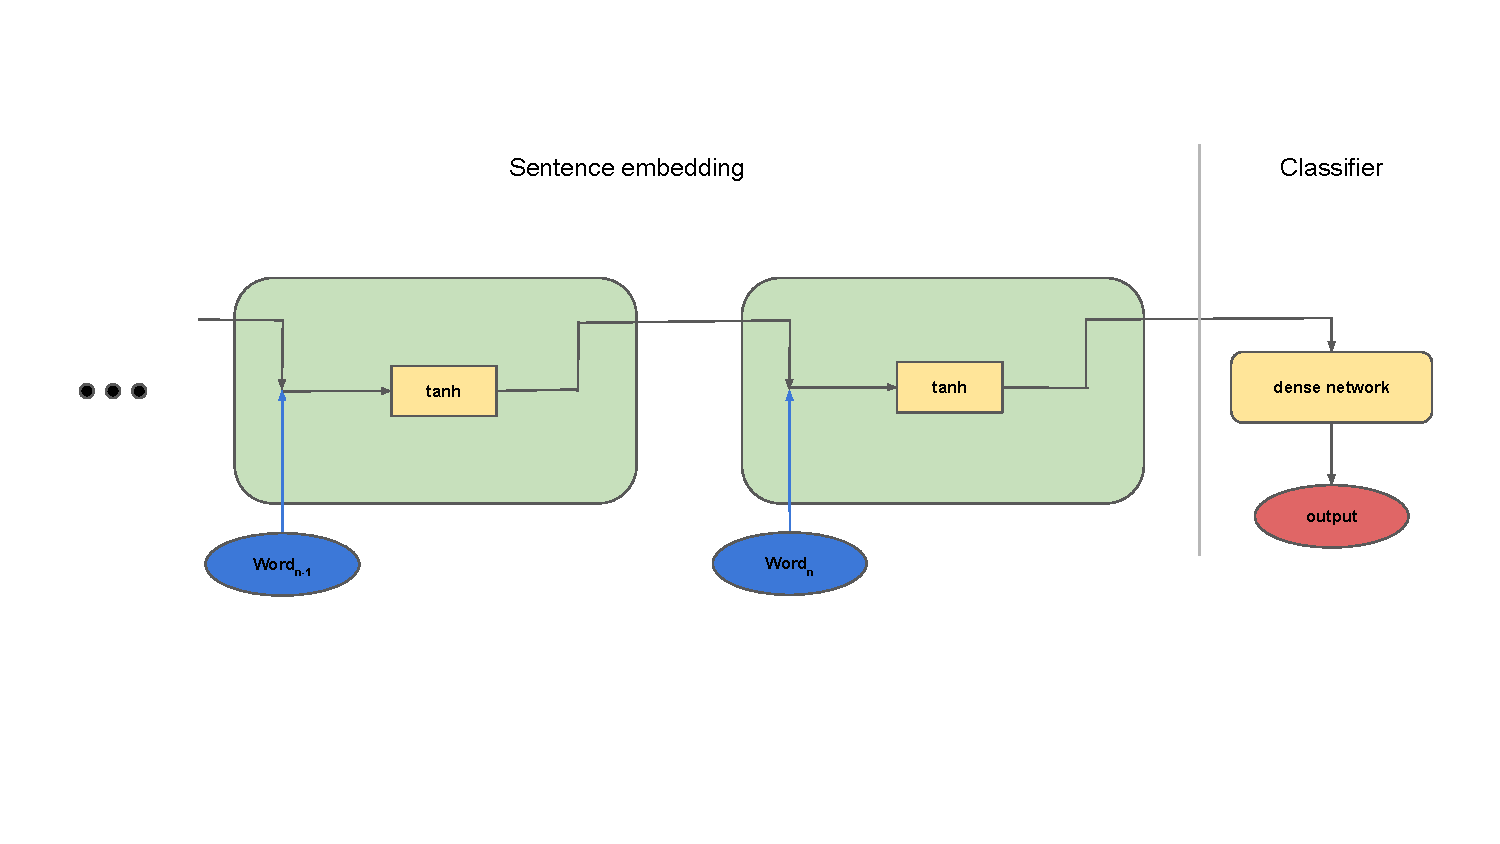
\includegraphics[width=\textwidth]{Images/Schema_RNN.pdf}
    \caption{Diagram of the iterative evaluation of a recurrent neural network in the language processing case. Only the two last iteration corresponding to the two last word of a sentence is represented. The green boxes represent several iteration of the same unit. The yellow rectangular boxes represent a single neuron layer and the rounded yellow box represent a dense network, which can made of several layers.}
    \label{fig:recurrent_network}
\end{figure}

The dense neural network that has been introduced is not well suited to our case. In order to use all the information available in jets, all the characteristics of the particles of each jet must be fed into the network. But each jet has a different number of particle, and a dense network cannot accommodate a varying number of inputs. Recurrent neural networks (RNN) are designed to accommodate such a varying number of inputs. They have been particularly useful in language processing tasks. Indeed, language processing have a similar varying number of inputs requirements, as the number of words changes in different sentences. RNNs are going to be introduced here in the case of an example task of classifying sentences as positive or negative.

Every RNN is composed of two distinct part, as illustrated in Figure \ref{fig:recurrent_network}. The first part has the goal of embedding the information gathered from the inputs into a fixed-size array of values, called the embedding array. The second part is a dense neural network that takes the elements of this array as input, and its output is considered the output of the RNN as a whole. The embedding part consists in applying a unit iteratively on each input element, in this case each word. The output of the previous iteration is also taken as a secondary input. The layout of a unit in terms of network layers and information flow then defines a specific RNN architecture.

While this architecture has the advantage of being able to accommodate inputs of varying size, it also benefits from the fact that the same embedding unit is applied at each iteration, with the same parameters. This mitigates the vanishing gradients problem, as all parameters of the network are evaluated close to the final layer. Conceptually, this allows the use of a small amount of layers by taking advantage of the symmetries of the inputs. 

\subsection{Recursive neural networks}
\label{sec:RecNN}


\begin{figure}
    \centering
    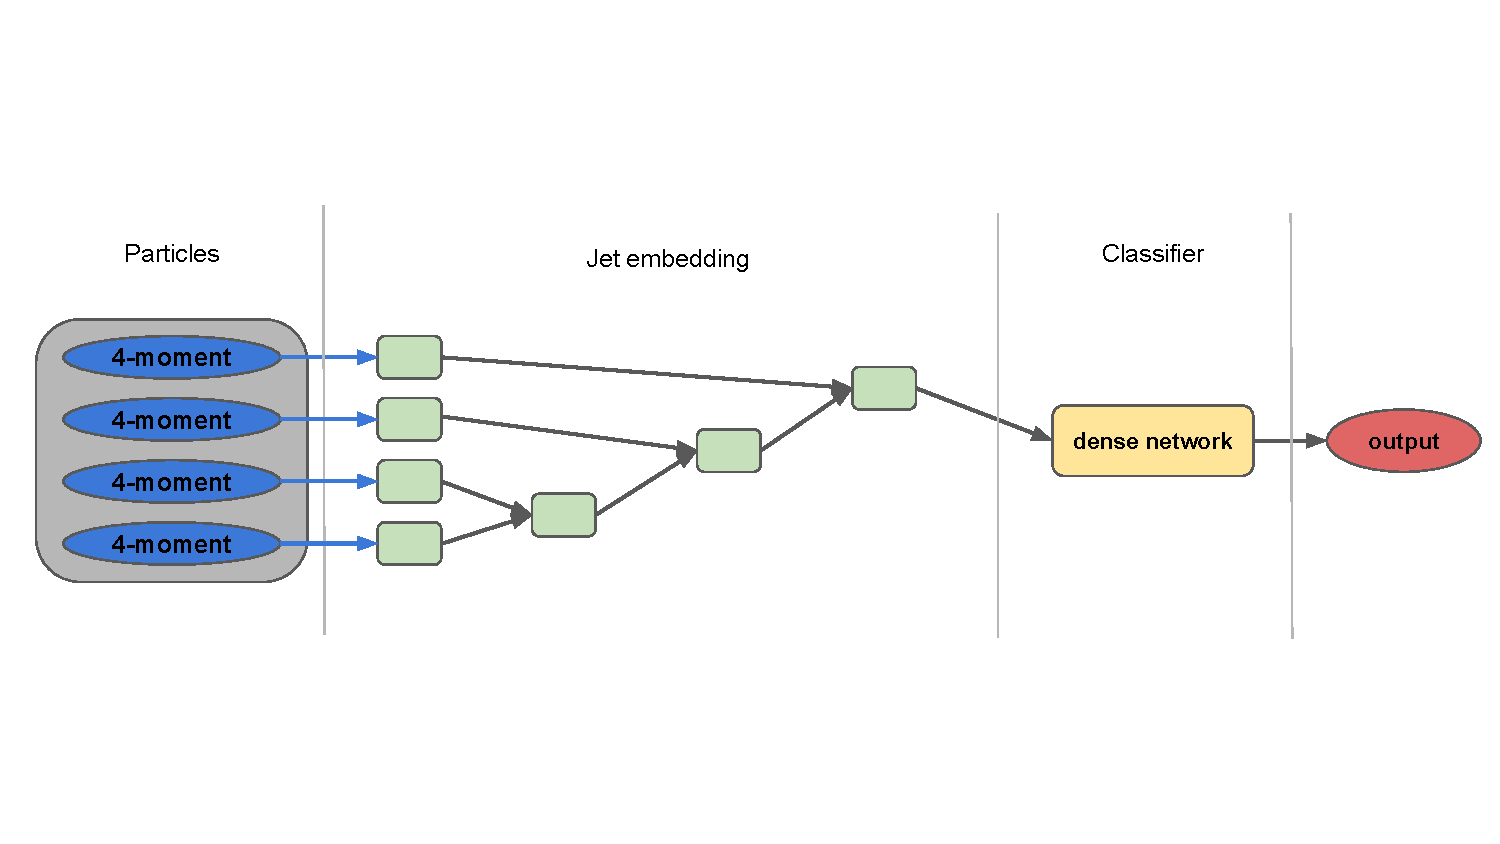
\includegraphics[width=\textwidth]{Images/RecNN_diagram.pdf}
    \caption{Diagram of the overall structure of the RecNN, including the jet embedding structure. The order in which the nodes are merged is determined by the chosen jet clustering metric. Each green box represents a node. Each node is evaluated with the same set of layer parameters. The black arrows represent the flow of both the 4-momentum and the embedding array. These arrows therefore represents both black and blue arrows from the node diagrams.}
    \label{fig:recursive_network}
\end{figure}

Similarly to how RNNs were designed to accommodate the needs of language processing, another architecture type has been designed to fit the needs of jet classification. This architecture type, called the recursive neural network (RecNN), was developed following the idea behind jet clustering. This architecture was first originally applied to the problem of boosted W-jet tagging \cite{Louppe:2017ipp}.

\subsection{Architecture}

As in a RNN, the network architecture is made of two parts, a jet embedding part and a final classifier consisting in a dense neural network. Contrarily to the linear structure of the sentence embedding, the embedding part is organized as a binary tree that represents the iterations of the jet clustering algorithm. The iterations of base units in a RecNN are called nodes. There are two types of nodes, namely the leaf nodes and the inner nodes. The leaf nodes are designed to each take the 4-momentum of an input particle, as illustrated in Figure \ref{fig:recursive network}. Inner nodes take the output of two other nodes, leaf or inner, as input. First, a criterion is evaluated on every pair of nodes, and the pair that best fulfill this criterion is selected. This criterion can be chosen among the following:
    
\begin{itemize}
    \item randomized : two nodes are selected at random;
    \item \pt-ordered : nodes holding the two pseudo-jets with the highest \pt;
    \item reversed \pt-ordered : the nodes holding the two pseudo-jets with the lowest \pt;
    \item $k_t$ : nodes holding the closest pseudo-jets following the $k_t$ clustering metric;
    \item Cambridge : nodes holding the closest pseudo-jets following the Cambridge clustering metric;
    \item anti-$k_t$ : nodes holding the closest pseudo-jets following the anti-$k_t$ metric.
\end{itemize}
The distance of two particles $i$ and $j$ in a clustering metric is defined as
\begin{equation}
    d_{ij} = \mathrm{min}(p_{Ti}^{2k},p_{Tj}^{2k}) \frac{\Delta_{ij}}{\mathrm{R}} \mend
\end{equation}
In this expression $\Delta_{ij}$ corresponds to the distance of the pseudo-jets in the ($\eta$,$\phi$) plane, R is a distance parameter, and $p_{Ti}$ corresponds to the modulus of the transverse momentum of particle $i$. The $k$ parameter is equal to 1 for the kt metric, 0 for the Cambridge metric, and $-1$ for the anti-kt metric.

Then, the output of the two chosen nodes are fed into an inner node. The 4-momentum associated to this new node is the sum of the 4-momenta of the two previous nodes, effectively creating a new pseudo-jet. The list of node is updated by removing the two merged nodes and adding the new inner node. The criterion is computed again for all pair combination and the process is repeated until only one node remains. The output of the final node is finally fed to the classifier part to provide a final output. 


\subsubsection{Node composition: gating}


\begin{figure}
    \begin{center}
    % \subfloat[RecNN leaf]{
        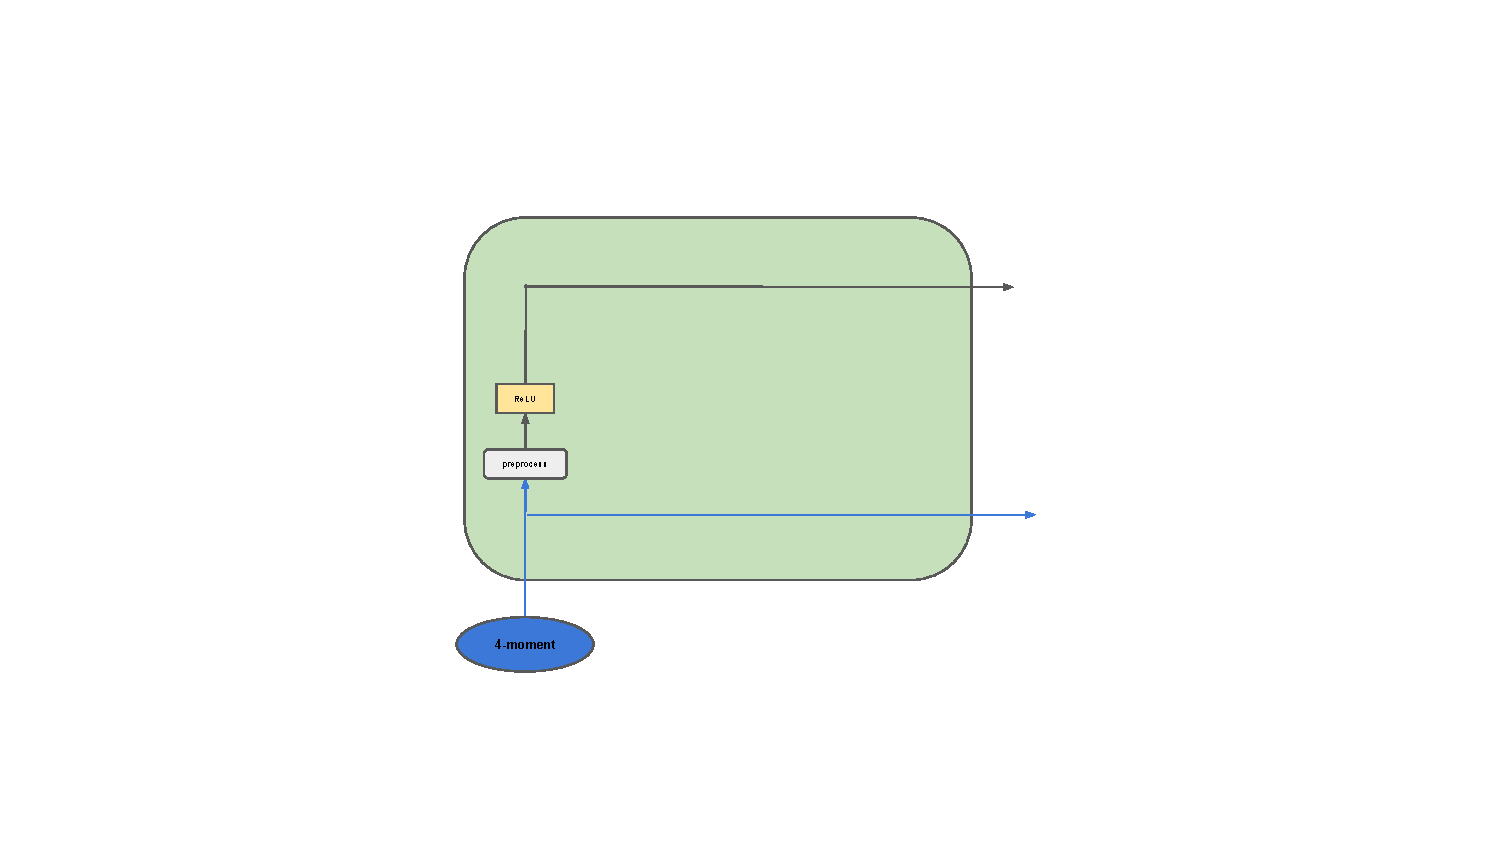
\includegraphics[width=\textwidth]{Images/Schema_RecNN_Leaf.pdf}
        \label{sub:RecNNLeafNode}
    % }
    
    % \subfloat[RecNN node]{
        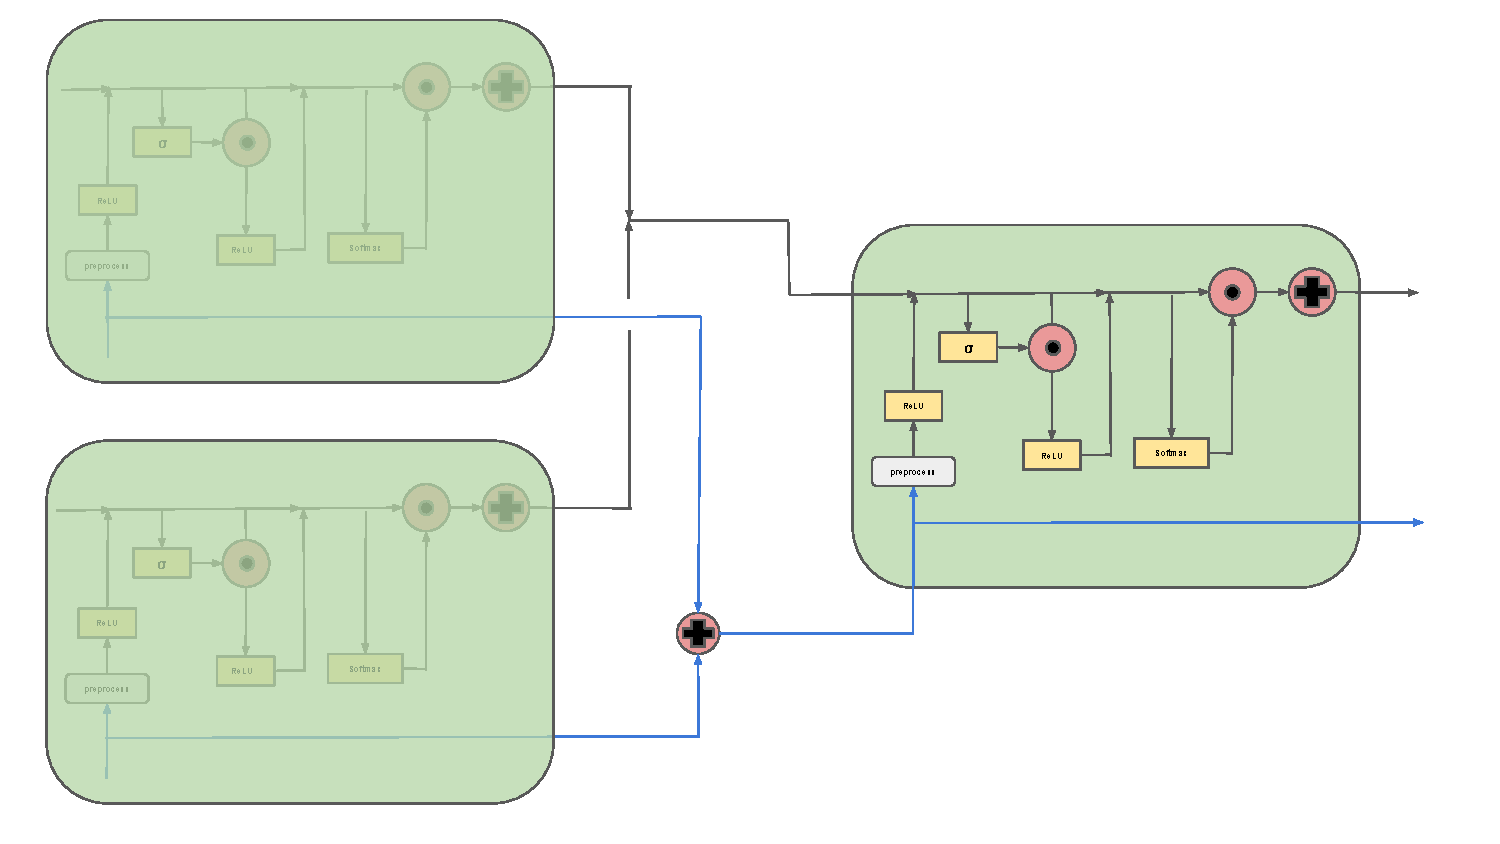
\includegraphics[width=\textwidth]{Images/Schema_RecNN.pdf}
        \label{sub:RecNNNode}
    % }
    
    % \subfloat{
    %     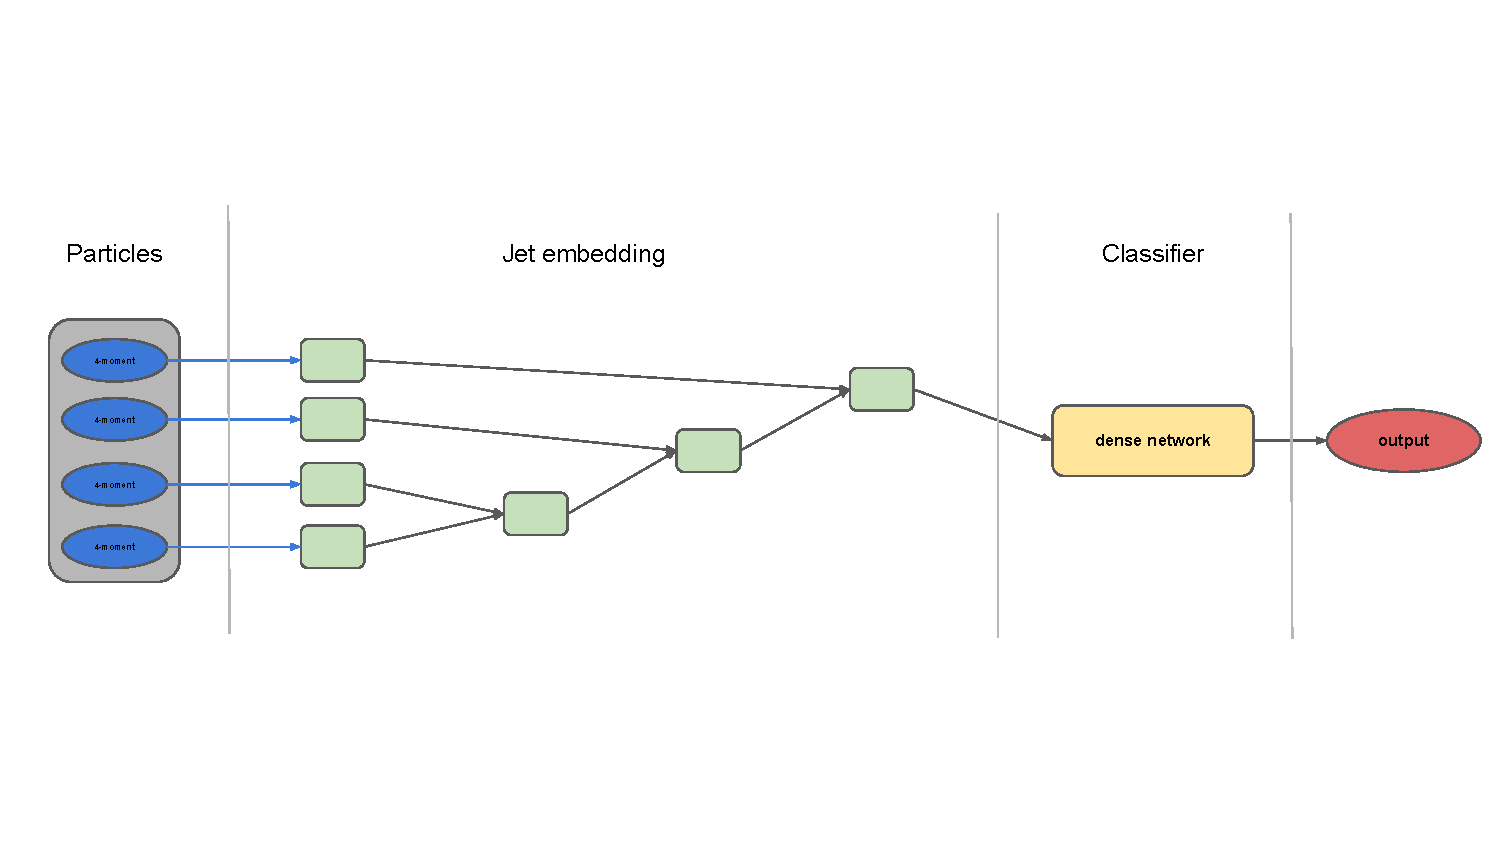
\includegraphics[width=\textwidth]{Images/RecNN_diagram_not_parall.pdf}
    %     \label{sub:RecNN_full}
    % }
    
    \caption{Diagrams of the nodes that can be found in a RecNN architecture. The top diagram represents a leaf node, which directly takes a particle 4-momentum as only input. The bottom diagram illustrates the inner structure of a node as well as how its input are taken from the previous nodes. The green boxes represent several iteration of the same unit. The yellow rectangular boxes represent a layer of neurons, and their names correspond to the activation function of the neurons in that layer. The blue arrows represent the path of 4-momentum merging at each iteration. The black arrow represent the path of the embedding arrays. The plus and dot signs in the red circles represent element-wise sum and element-wise product, respectively. The white box represent the preprocessing step that involves the transformation into cylindrical coordinates, as well as the scaling of each variable.}
    \label{fig:recnn}
    \end{center}
\end{figure}

Similarly to a RNN, the role of a inner(leaf) node is to modify(create) an embedding array. An inner node layout therefore takes two inputs, namely the 4-momentum of a pseudo-jet and an embedding array. While the 4-momentum is then directly given as output for the next node, the embedding array will be modified through the use of one or several neuron layers. Thus, the information effectively takes two parallel paths. Indeed, a first path is defined by the propagation of the 4-momenta, while a second path is defined by the merging and modifications of embedding representation arrays. 

While several node layouts are tested in \cite{Louppe:2017ipp}, the gated layout has the best results and is the basis of our version. Inspired by the long short-term memory (LSTM) architecture \cite{lstm} and gated recurrent unit (GRU) architectures \cite{GRU}, the gating conceptually adds the possibility for the network to select and mix available information more easily. While a mathematical formulation of this layout is available in the appendix of the article, the following explanation relies on the illustration in Figure \ref{fig:recnn}. 

First, each leaf node takes the 4-momentum of a particle and directly propagates it as its secondary output. A copy of this 4-momentum is preprocessed in two distinct steps. In the first step, the 4-momentum expression is changed from the easily addable Cartesian coordinates, to the more interpretable spherical coordinates. A few more variables are also computed at this step, like the modulus of the momentum $p$ and the mass $m$. Each of those variables are then scaled by the robustScaler method \cite{robustscale} trained on the whole dataset. The goal of this scaling is to make the distributions of all variables comparable in terms of median and quantiles. Conceptually, this avoids the following layers to be forced to learn the scales of each variable. 

The output of this preprocessing step is given as input to a first ReLU layer. The output array of this layer, designed to be of the same shape as each of the two input embedding arrays, is concatenated with these arrays. A second ReLU layer is evaluated by combining the information in this new embedding array using a reset gate. Conceptually, the goal of this reset gate is to actively select which parts of the embedding array are to be emphasized, and which parts are to be forgotten. This reset gate is implemented by evaluating a sigmoid layer, which takes as input the embedding array and creates an output array of the same shape, with values between 0 and 1. An element-wise product between the output array and a copy of the embedding array is then computed before feeding the produced array into the second ReLU layer. The output of this second ReLU layer, designed to have the same shape as the input embedding arrays, is then also concatenated to the new embedding array.

At this point the embedding array consists of the concatenation of four different arrays of the same shape: two embedding arrays outputs from the previous nodes, a local evaluation of the pseudo-jet, and an array produced from the combination of all the previous ones. In order to combine all those information into an array of the desired shape, a softmax gate is applied. This softmax gate is designed to weight each variable of the embedded array by a scalar, before the four concatenated arrays are added element-wise. These weights are determined by a softmax neuron layer. The output weights $w_i$ of this softmax layer are determined from the activation of each output neuron $Z_i$ by
\begin{equation}
    w_{i} = \frac{e^{Z_i}}{\sum_{j=1}^{K}e^{Z_j}} \mend
\end{equation}
The product of this softmax gate is then the embedding array output of this node. If the node is the final node, this output is then directly fed into the dense neural network classifier part of the architecture.

\subsubsection{Jet centering}

The position of the jet in the detector impacts all the variables, while having little to do with the identification process. To avoid adding the task of learning this fact, the reconstructed jets are centered around the highest \pt particle. After centering particles appear to the network as orientated around the center (0,0) of the ($\eta$,$\phi$) plane. The jet is then re-clustered into three subjets. Jets are finally rotated and if needed mirrored so that the the positions of the re-clustered subjets are similar in every jet.

\section{Recursive neural network for hadronic tau decay identification}


% \begin{figure}
%     \centering
%     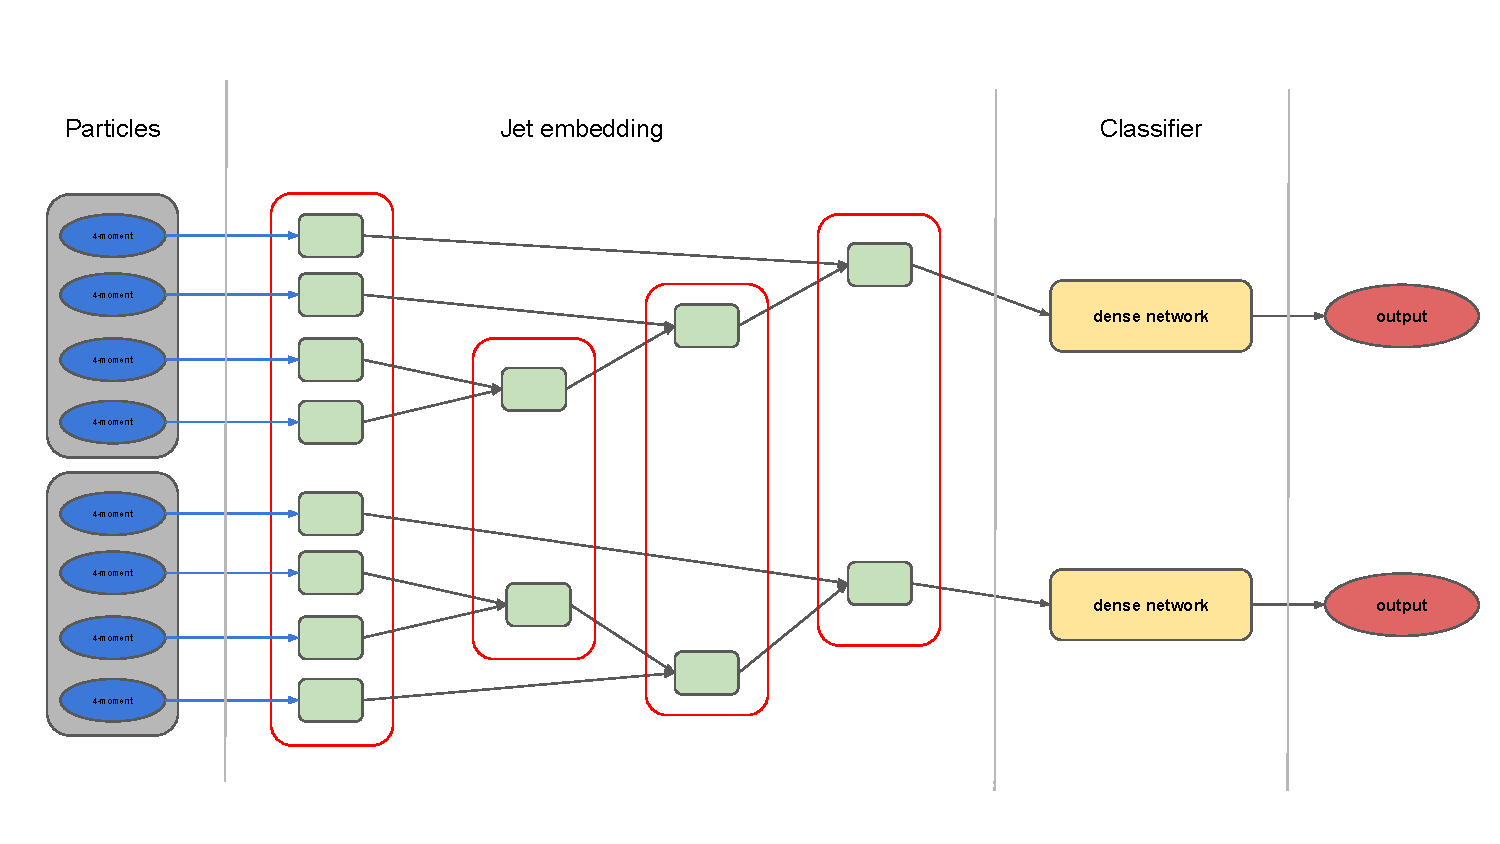
\includegraphics[width=\textwidth]{Images/RecNN_diagram_parall1.pdf}
%     \caption{Illustration of the parallelisation of computing in the RecNN. The red boxes correspond to node-depth levels that are evaluated and trained simultaneously in a single mini-batch.}
%     \label{fig:RecNN_parall}
% \end{figure}



\subsection{Implementation}

While most neural network architectures can easily be implemented using widely available libraries like Keras \cite{chollet2015keras}, the RecNN architecture cannot be implemented from these libraries, mainly because of its changing structure that adapts to each jet. The RecNN architecture was therefore implemented by the authors of Ref. \cite{Louppe:2017ipp} with classes from the scikit-learn library \cite{scikit-learn} as a base. We started from this implementation. 

The first difference brought by our implementation is purely an optimization of the code. While the code was already designed to run in parallel on several cores at the evaluation and training phases, both the preprocessing and centering steps were not. By adapting those steps and running in parallel the time needed for this step was reduced from several hours to about $15\,\mathrm{min}$ using $20$ cores. Time was also gained by changing the format under which the arrays were saved on disk.

In order to compare the standard and RecNN methods and to study score distributions on population subsets, the code was adapted to be able to track jets through the evaluation process. Indeed, in the original code the formatting of particles into the arrays used as input to the RecNN meant the loss of its link with any other information, such as the score of the jet with the standard technique, or the gen-level information. This tracking also allowed to build a display of jets with their associated gen-level information, allowing a case-by-case study.

\subsection{Upgrade}

In the original implementation, particles are described only by their 4-momentum. But the nature of those particles as well as other available information was not used. In order to add this information, the 4-momentum was changed to an array holding extra information. Just like the 4-momentum, the extra information must consist of variables that can be added when merging two nodes.

The first variables added are the energy and \pt contributions to the pseudo-jet from each particle type, namely photons, electrons, muons, neutral hadrons, charged hadrons from the primary vertex, and charged hadrons from pileup. Charged hadrons are considered as coming from the primary vertex if the distance between the primary vertex and the closest point of their reconstructed trajectory is found to be less than $0.2\,\mathrm{cm}$ away from the primary vertex along the z-axis.

As the number of particle of each type is relevant to identify the different \tauh decay modes, the total number of each particle type in a given pseudo-jet is also added.

\subsection{Performance}

\begin{figure}
    \centering
    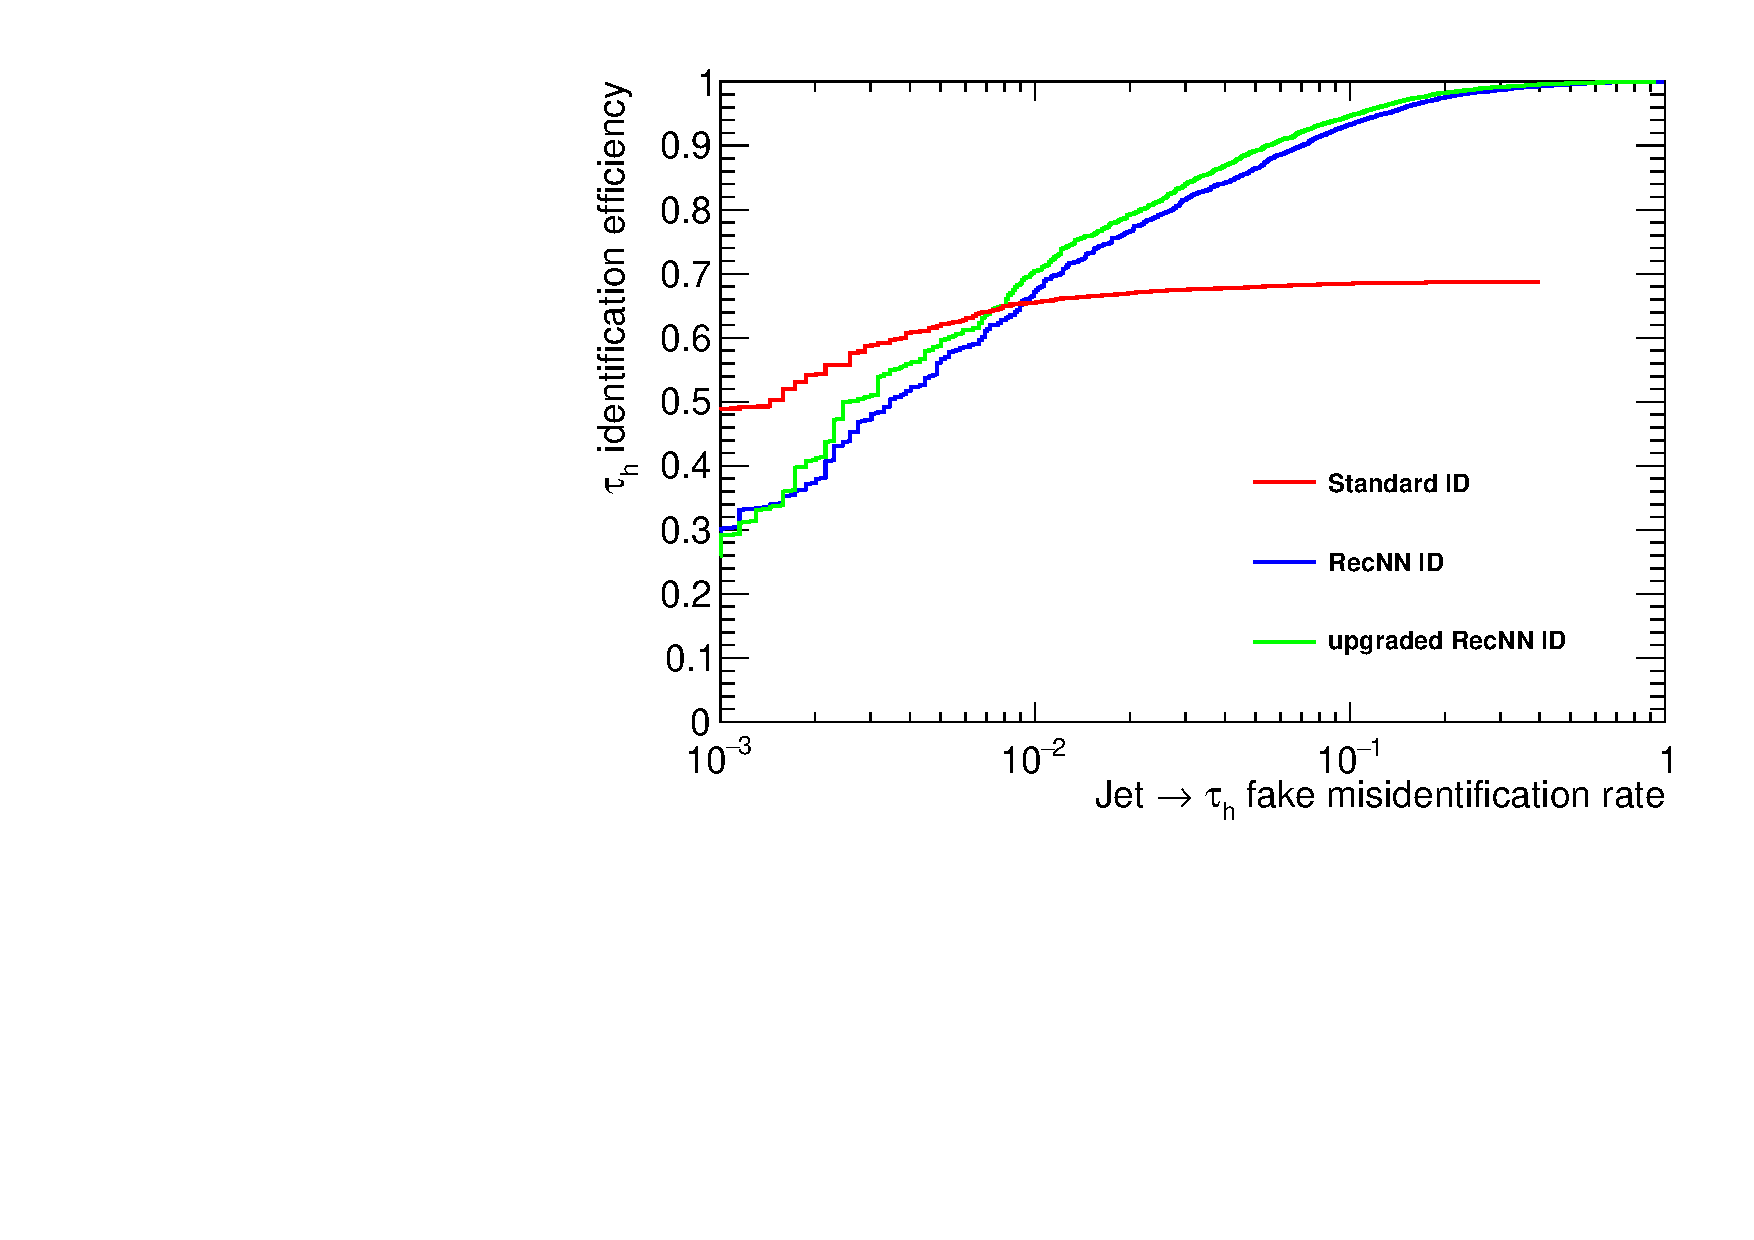
\includegraphics[width=\textwidth]{Images/ROC_comp_all.pdf}
    \caption{\tauh identification ROC curve for the standard method, the RecNN method, and the upgraded RecNN method. The x axis is set to a logarithmic scale.}
    \label{fig:RecNN_ROC}
\end{figure}

The ROC curves of both the standard method, the base RecNN implementation and the upgraded RecNN approach are presented in Figure \ref{fig:RecNN_ROC}. While the area under the curve is strictly better in the RecNN approaches compared to the standard method, the efficiency of the standard method is still better at low jet misidentification rate. The gain from the upgrade of the RecNN, while significant, is less than expected. 


\subsection{Possible optimization}

Although the results have shown some potential, this study has not reached the level of optimization that could help the RecNN to outperform the standard technique systematically. Indeed, several upgrades that could benefit the RecNN approach have been considered, but were not fully implemented in time. 

Even while limiting as much as possible the computational times, the latest versions of the RecNN network have proven to be long to train, about two days on a dedicated machine with 40 cores. All the clustering orderings have shown similar results in several stages of optimization. While all should be optimized and tested eventually, the presented results have been produced with the anti-$k_t$ ordering.


\begin{figure}
    \centering
    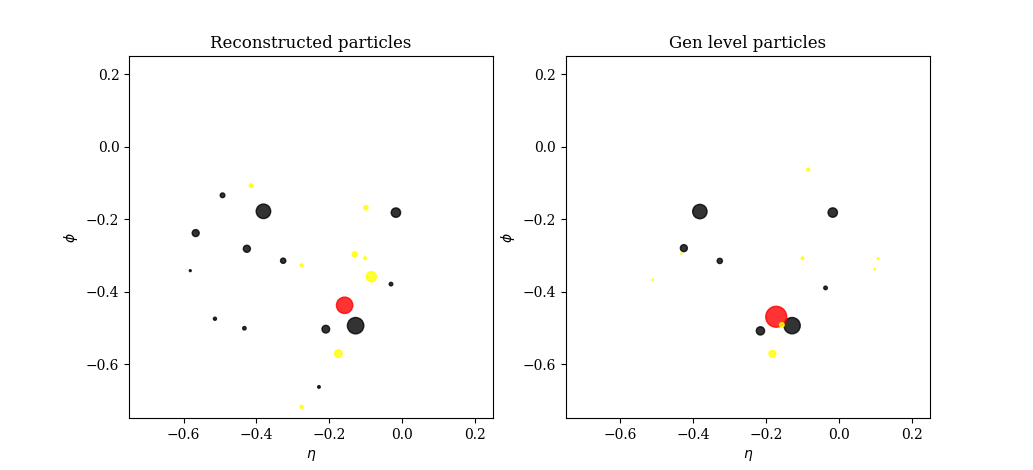
\includegraphics[width=\textwidth]{Images/mistaggedQCD.png}
    \caption{Scatter plots of the particle constituents in a QCD jet misidentified by the RecNN network. Top: reconstructed jet. Bottom: gen-level jet. The size of the points are proportional to the \pt of the particles and their color depends on their type. Black points represent charged hadrons, yellow represent photons and red represent neutral hadrons.}
    \label{fig:jet_display}
\end{figure}


One such upgrade idea came from the study of QCD jets misidentified by the RecNN. Indeed, many examples such as the QCD jet mistagged as a \tauh by the RecNN network displayed in Figure \ref{fig:jet_display} show cases where the RecNN should be able to classify such QCD jets as background from the number of reconstructed charged hadrons. These observations imply that the RecNN approach does not use the number of particle information as efficiently as it should. An upgrade would be to directly add the number of particle per type at the classifier-level, rather than the jet embedding level. This could help the network to easily reject trivial cases, while being able to specialize the jet-embedding part for the less straight-forward cases.

In our training sample, a majority of QCD jets can be trivially rejected from the number or composition of reconstructed particles. This implies that most training cases are not useful for the network. Conceptually, this means the only useful training is done an a subset of examples, while the other training cases only contribute to an effect called overtraining. This effect appears when the networks learns characteristics that are specific to the training sample, but those characteristics are not generalizable. To avoid this overtraining, the training phase is stopped when performances measured on an independent sample starts getting worse as the training continues. A possible change to be tested could be to select more QCD jets that are similar to \tauh products in the training sample, and select less trivial cases.

While all those optimizations were attempted, these were not implemented in time. The RecNN approach has shown good performances already, and while the implemented upgrades have improved these performances, further improvements are expected to be within reach, as the case-by-case study shows. The potential optimization that were discussed could help reach a better performance.